\chapter{Үр дүн}

Дээрх хэрэгжүүлэлтийн үр дүнд дараах зургуудад харагдаж байгаачлан манай веб апп маань ашиглахад бэлэн болсон. Доор гол гэсэн хуудсуудын ажиллаж буй процессыг илэрхийлэх хуудсуудын зургуудуудыг оруулав.

\begin{figure}[h]
	\centering
	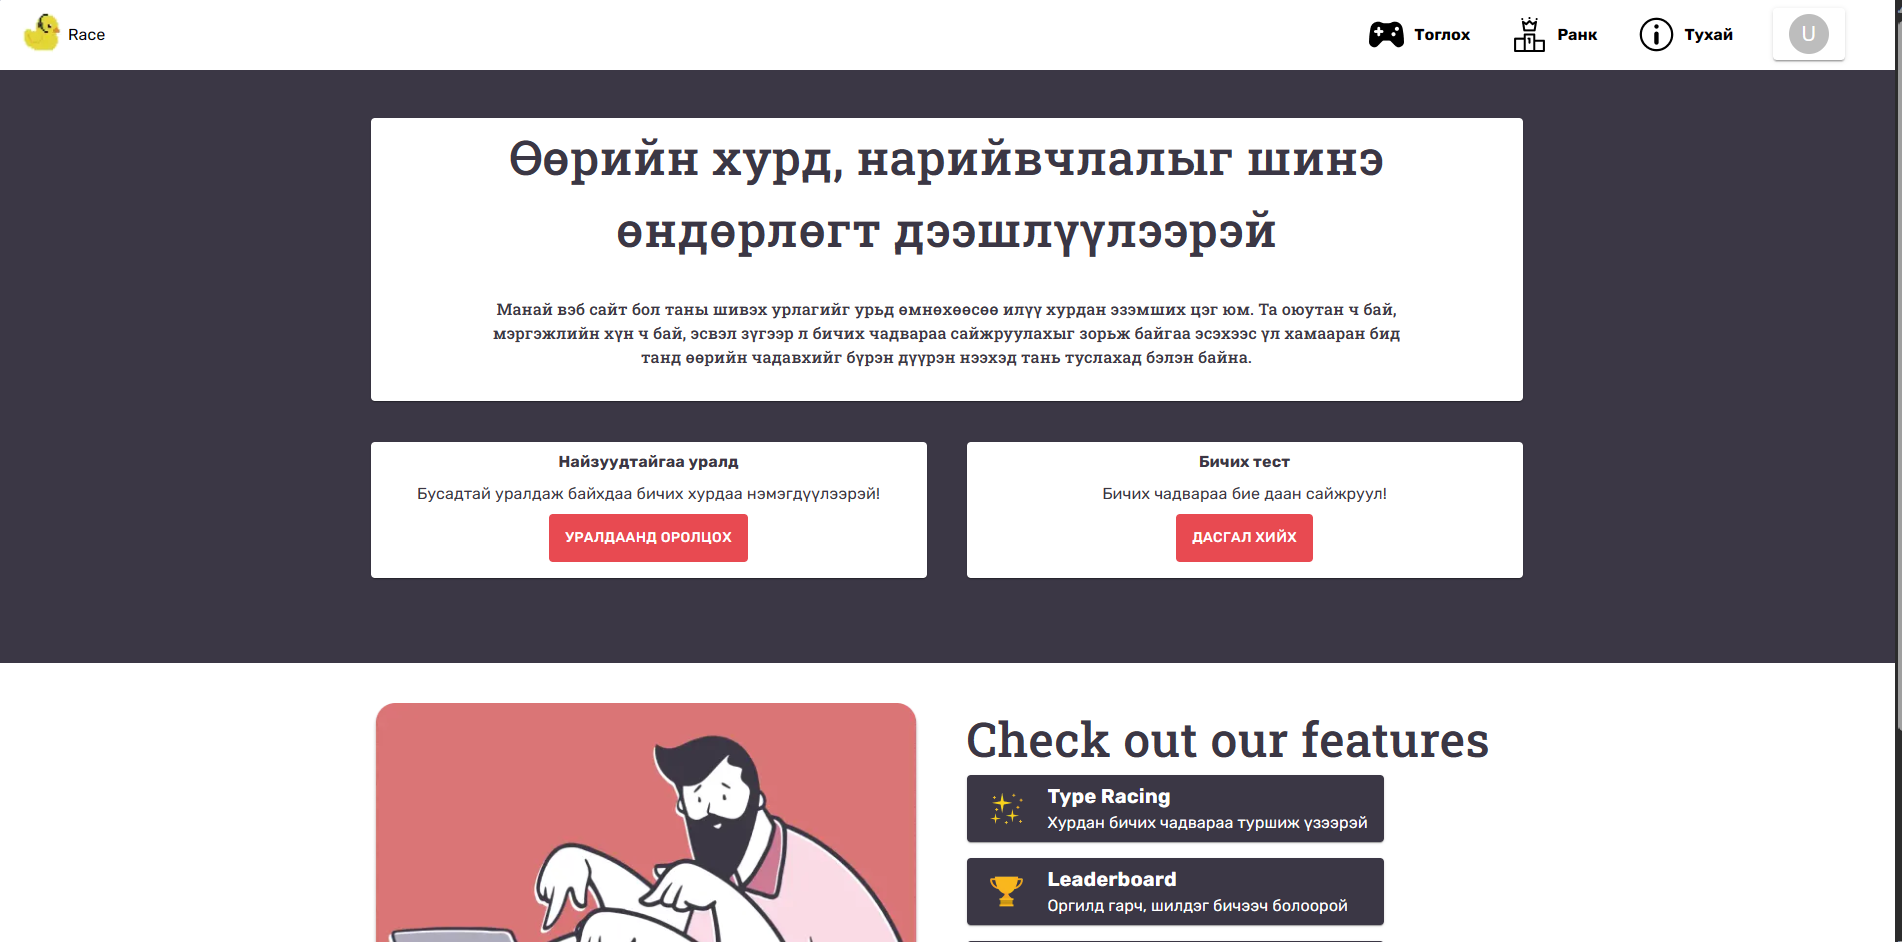
\includegraphics[width=13cm]{images/result/homepage.png}
	\caption{Нүүр хуудас}
	\label{fig:results}
\end{figure}

\begin{figure}[h]
	\centering
	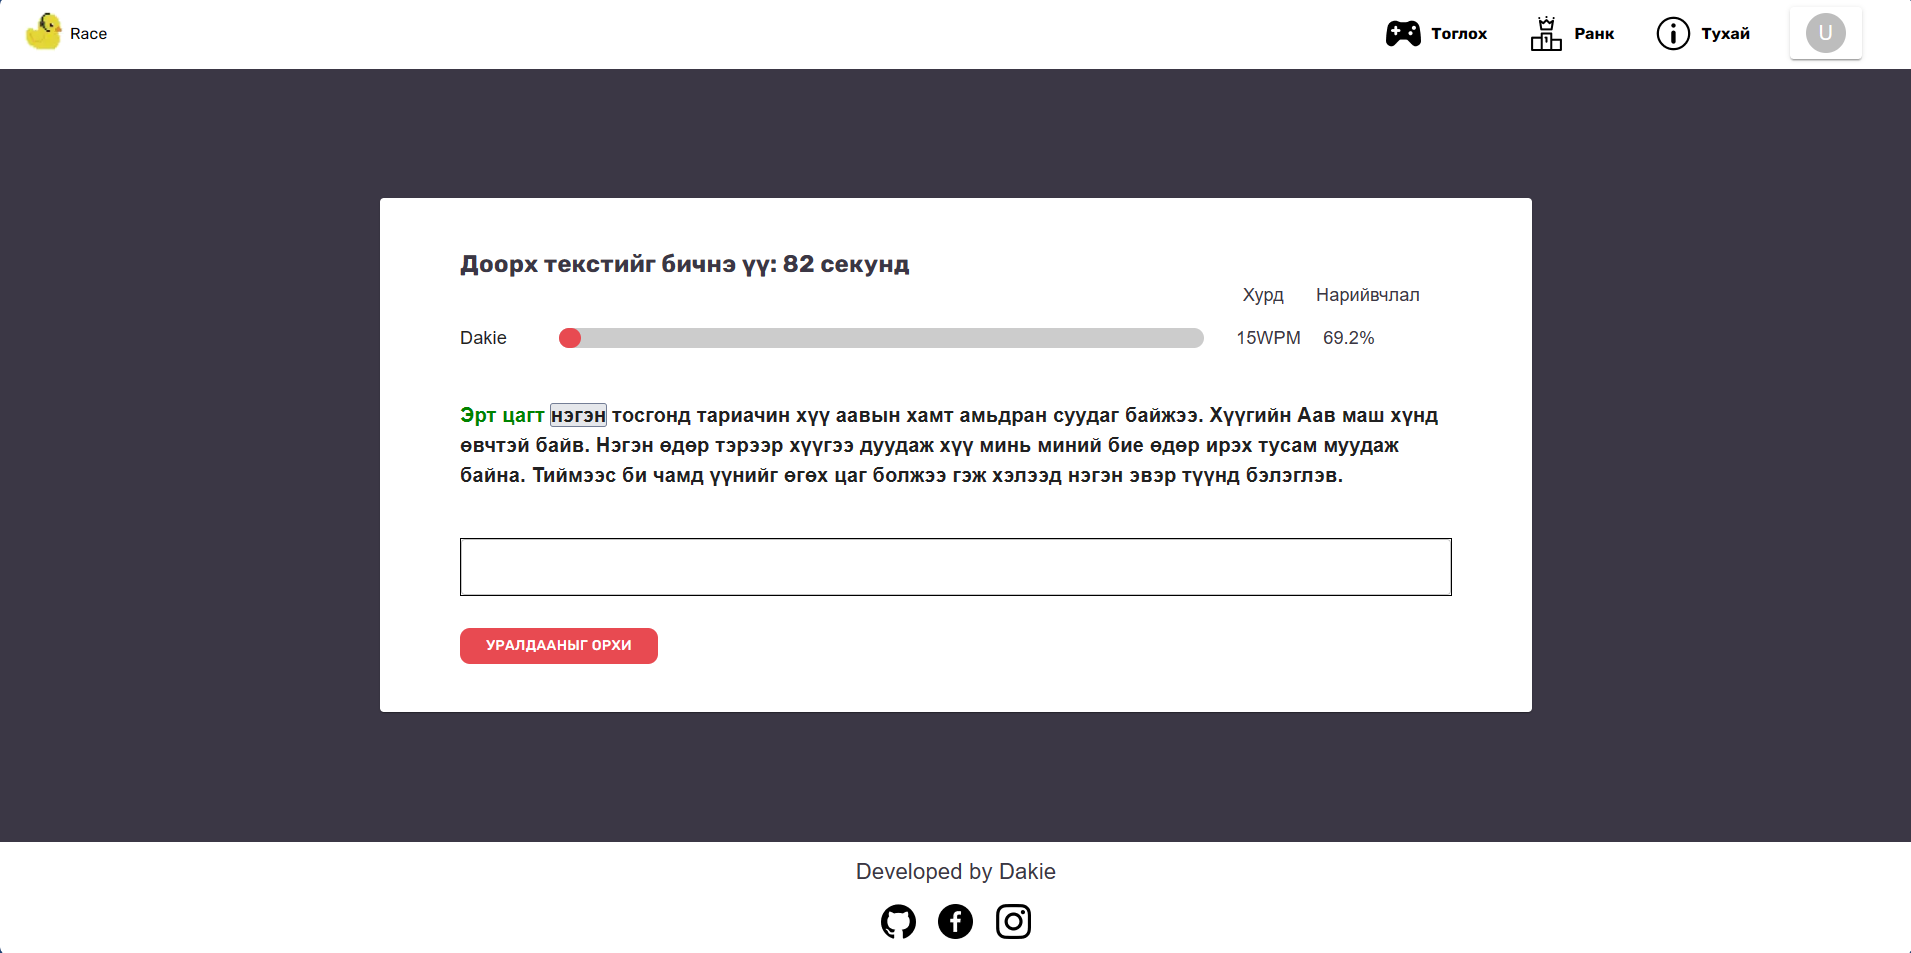
\includegraphics[width=13cm]{images/result/playpage.png}
	\caption{Хэрэглэгч шивэх тест өгөх хуудас}
	\label{fig:results}
\end{figure}

\begin{figure}[h]
	\centering
	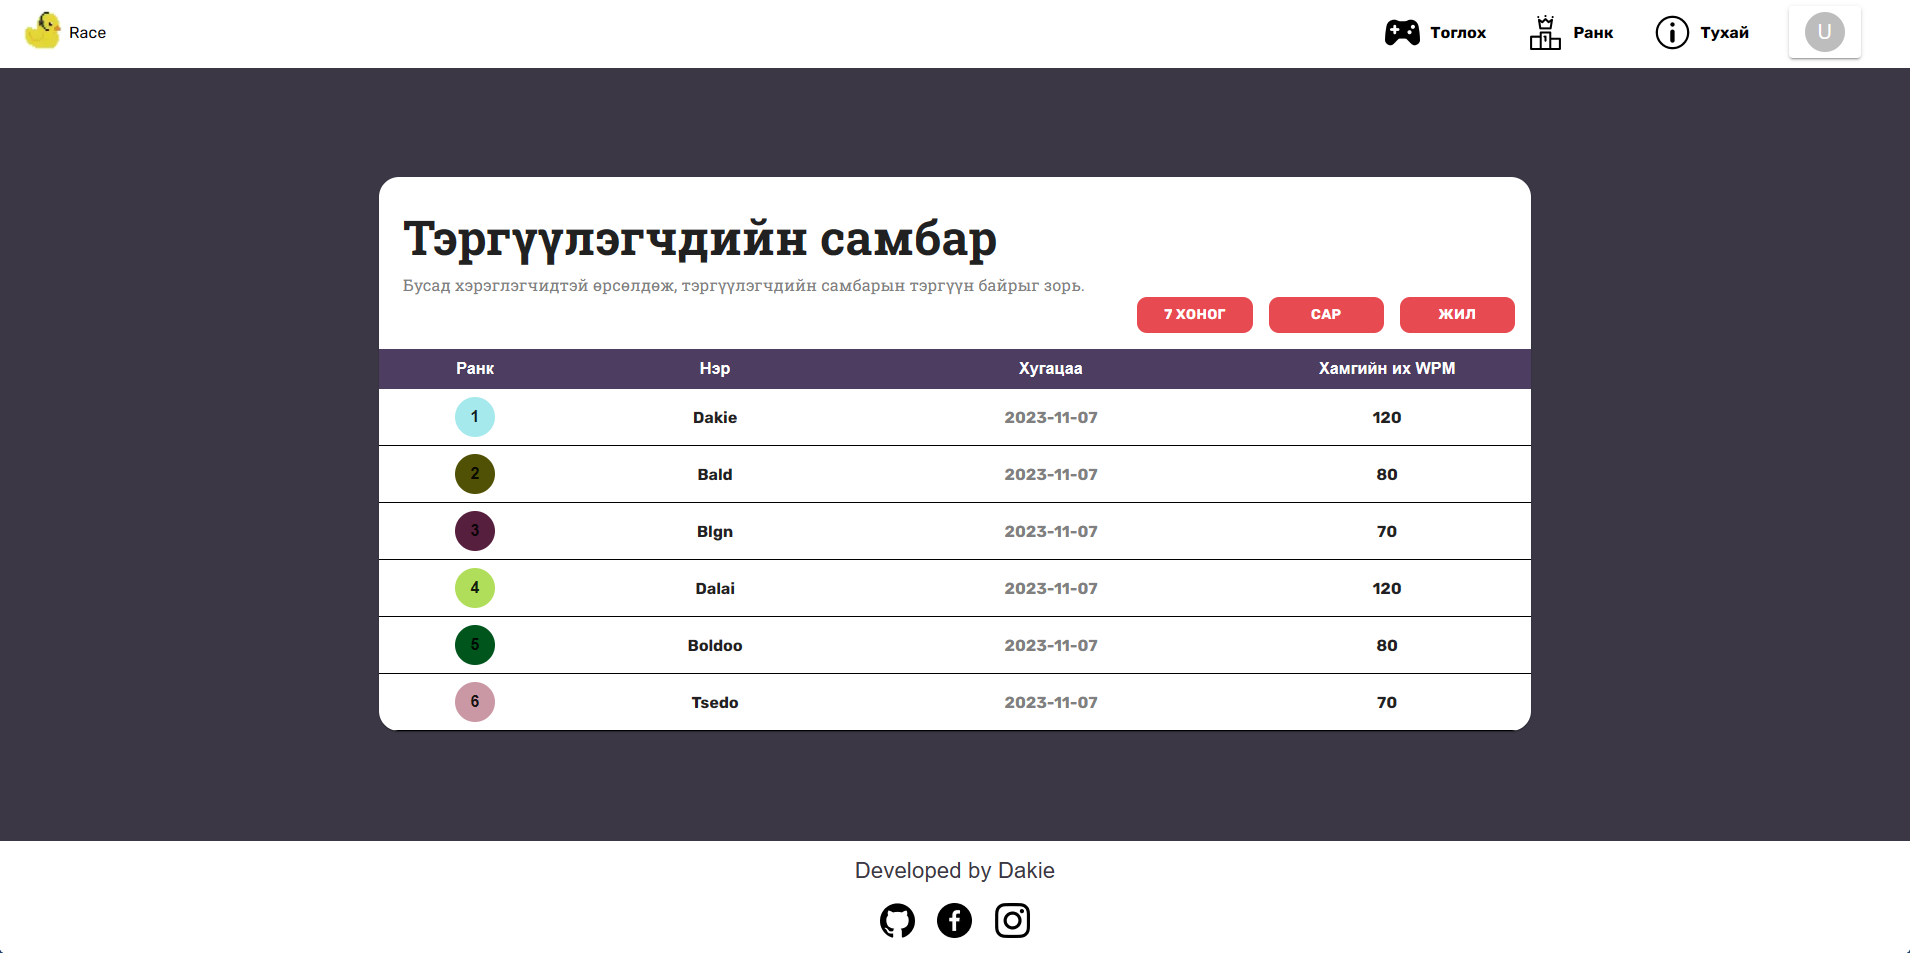
\includegraphics[width=13cm]{images/result/rankpage.png}
	\caption{Нийт тоглогчдыг тэргүүлэгчдийн хуудас}
	\label{fig:results}
\end{figure}

\begin{figure}[h]
	\centering
	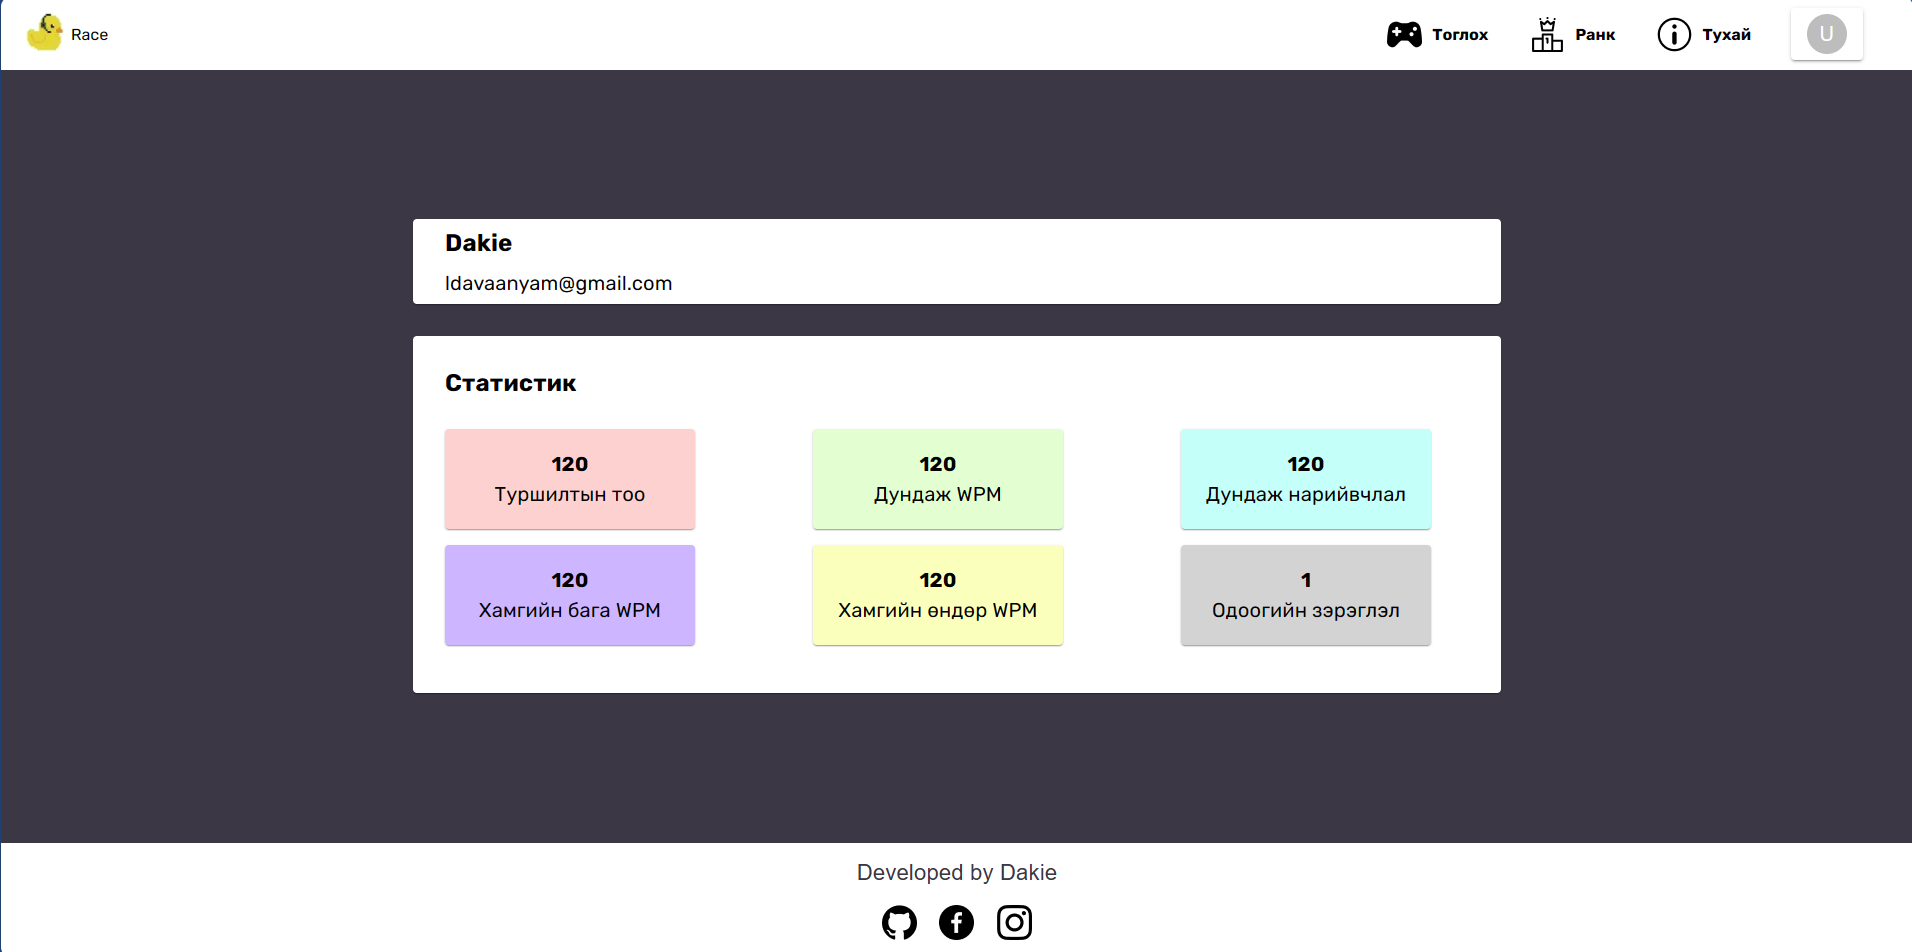
\includegraphics[width=13cm]{images/result/statisticspage.png}
	\caption{Хэрэглэгчийн статистикийн хуудас}
	\label{fig:results}
\end{figure}

\begin{figure}[h]
	\centering
	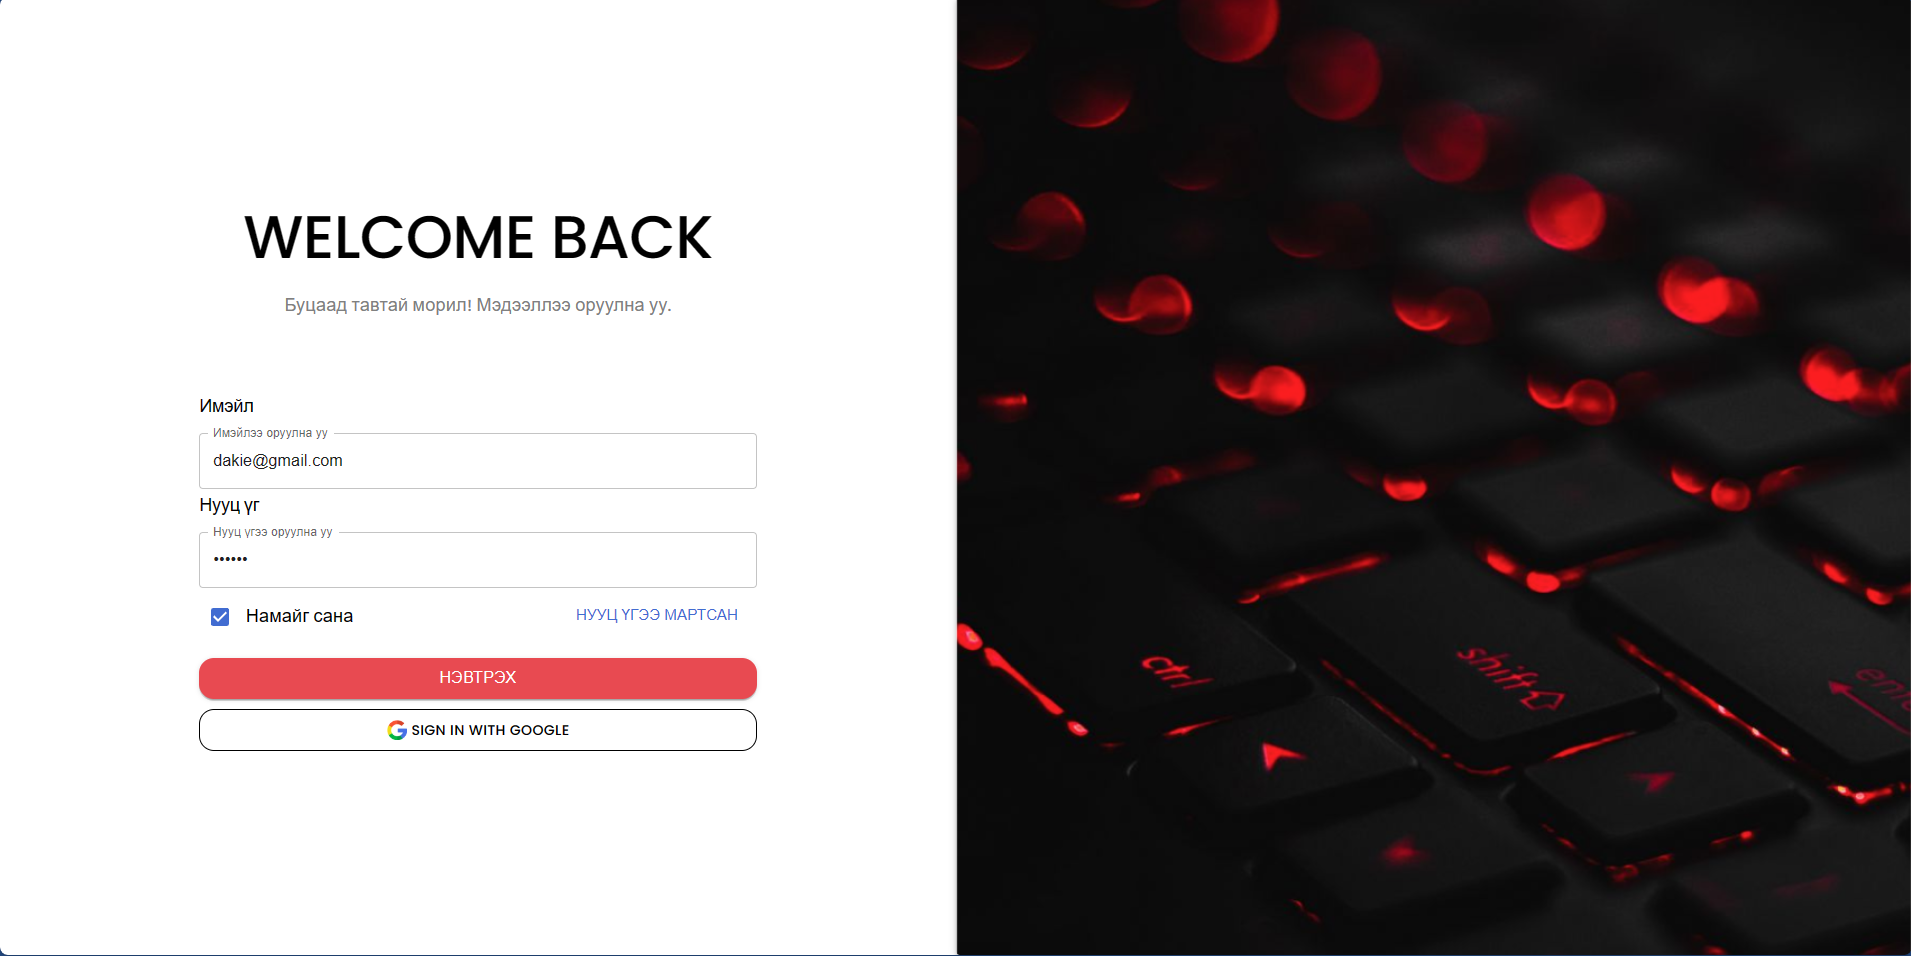
\includegraphics[width=13cm]{images/result/loginpage.png}
	\caption{Нэвтрэх хуудас}
	\label{fig:results}
\end{figure}

\begin{figure}[h]
	\centering
	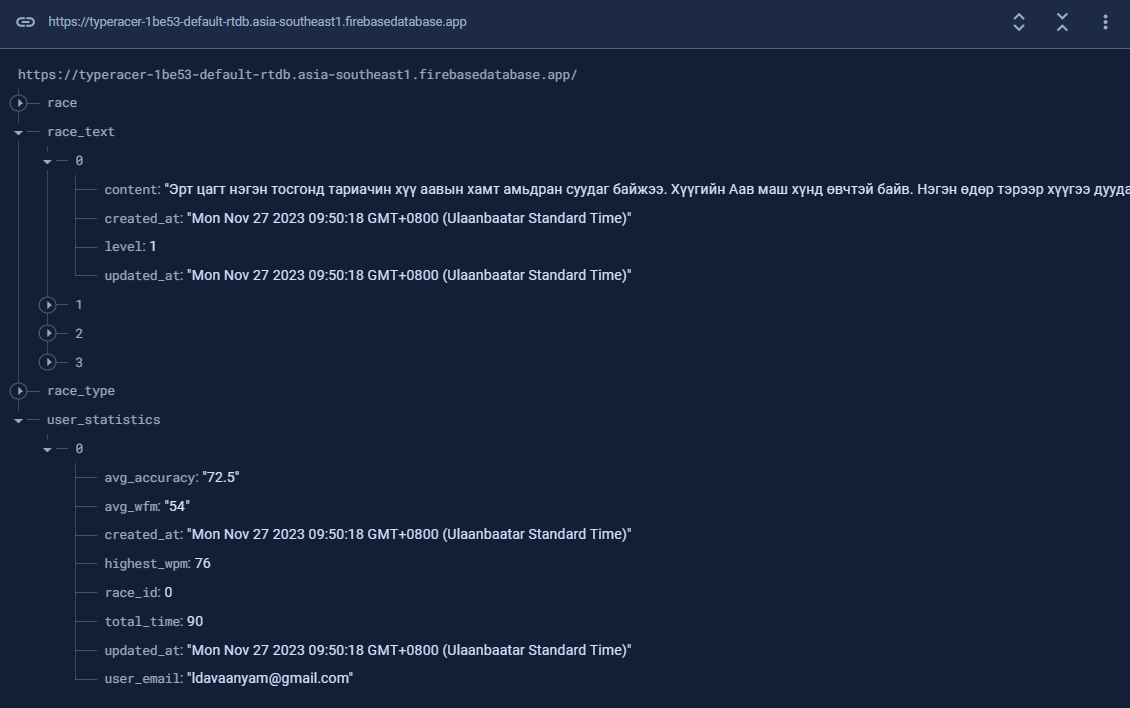
\includegraphics[width=13cm]{images/result/firebase.png}
	\caption{ Firebase realtime өгөгдлийн бааз хянах цонх}
	\label{fig:results}
\end{figure}